\chapter{Kriging-Based Navigation}

\vfill
\localtableofcontents
\vfill
\newpage

\section{Introduction}

Assume a navigation scenario similar to that of \cref{sec:Bayesian_estimation}:
\begin{equation}
	\left\{\begin{aligned}
	x_k&=f_k(x_{k-1},w_k)\\
	z_k&=h_k(x_k,n_k)
	\end{aligned}\right.
\end{equation}
with the exception that $h_k$ is unknown, and the observation noise is additive for the sake of simplicity. Since the likelihood density cannot be evaluated without an observation model, Bayesian data fusion is no longer applicable, and we may only rely on inertial navigation to estimate the state $x_k$.

In our scenarios, the observation function describes the measurement of a physical field, which does not change over the course of the mission, by an embedded sensor at each time step. Furthermore, we assume that the environment has been sampled before the mission, whether during a previous reconnaissance mission, or using a known but deteriorated map. This is formally modelled by \cref{th:kriging_navigation_assumptions}.

\begin{assumption}[Observation model]\label{th:kriging_navigation_assumptions}
	The observation function is a time-invariant GP, and its noise is an additive Gaussian white noise of covariance matrix $R_k\succeq0$:
	\begin{equation}
		z_k=h(x_k)+n_k,\qquad n_k\sim\mathcal{N}(0,R_k)
	\end{equation}
	where $m:\mathbb{R}^{d_x}\to\mathbb{R}^{d_z}$ is the potentially unknown mean of the GP, and $k:\mathbb{R}^{d_x}\times\mathbb{R}^{d_x}\to\mathbb{R}^{d_z}$ is its chosen covariance kernel. Here, $n_k$ plays the role of the query noise $\varepsilon$ of \cref{sec:kriging}, and $R_k$ is its associated covariance $R$.

	We also have access to $\tilde{n}\in\mathbb{N}^*$ distinct training inputs $\tilde{\mathbf{x}}$ and their noisy observations $\tilde{\mathbf{z}}$, degraded by a noise of covariance $\tilde{R}\succeq0$, in the sense of \cref{sec:kriging}.
\end{assumption}

\begin{remark}[Time-varying observation function]
	In full generality, the observed physical field could vary over time, and so the underlying GP would need to include a temporal input. While the kriging theory perfectly works with this additional parameter, it would require the training data to be sampled over time as well as space.
\end{remark}

This chapter is organised as follows:
\begin{itemize}
	\item \Cref{sec:kriging_PF} combines \cref{sec:Bayesian_estimation,sec:Gaussian_processes} to create a kriging-based framework for autonomous navigation in a poorly-known environment.
	\item \Cref{sec:AK_PF} discusses non-stationary observation fields, and the necessity of training data selection for kriging.
	\item \Cref{sec:CAK_PF} improves upon this framework by clustering the particle cloud to better capture the non-stationarities of the field.
	\item Finally, \cref{sec:subsampling_error} quantifies the estimation error committed by subsampling the training data used for kriging.
\end{itemize}

\section{Kriging the Observation Model}\label{sec:kriging_PF}

Using \cref{th:kriging_navigation_assumptions}, the likelihood follows:
\begin{equation}
	z_k|x_k,\tilde{\mathbf{z}}\sim\mathcal{N}\left(\hat{z}_{\mathrm{K}}(x_k,\tilde{\mathbf{x}},\tilde{\mathbf{z}};m,g),R_{\mathrm{K}}(x_k,\tilde{\mathbf{x}};g)\right)\label{eq:kriged_likelihood}
\end{equation}
where $\hat{z}_{\mathrm{K}}$ denotes any of the three kriging estimators, $R_{\mathrm{K}}$ is the corresponding covariance matrix, and $m$ and $g$ are optional arguments depending on the chosen kriging method. In particular, $R_{\mathrm{K}}$ already carries the query noise $R_k$, so it must not be added a second time.

\textbf{TODO: à reprendre}
\begin{remark}[Correlated map error]\label{th:correlated_map_error}
	The filtering recursion does not call for \eqref{eq:kriged_likelihood}, but for $p(z_k|\mathbf{x}_{0:k},\mathbf{z}_{1:k-1},\tilde{\mathbf{z}})$. Marginalising over the field, then using that the observation noise is white once $h$ is given:
	\begin{equation}
		\begin{aligned}
		p(z_k|\mathbf{x}_{0:k},\mathbf{z}_{1:k-1},\tilde{\mathbf{z}})&=\int{p(z_k|\mathbf{x}_{0:k},\mathbf{z}_{1:k-1},\tilde{\mathbf{z}},h)\:p(h|\mathbf{x}_{0:k-1},\mathbf{z}_{1:k-1},\tilde{\mathbf{z}})\:dh}\\
		&=\int{p(z_k|x_k,h)\:p(h|\mathbf{x}_{0:k-1},\mathbf{z}_{1:k-1},\tilde{\mathbf{z}})\:dh}
		\end{aligned}
	\end{equation}

	The first factor is the one \eqref{eq:kriged_likelihood} uses as well. The second is not: $\mathbf{z}_{1:k-1}$ are noisy evaluations of $h$ at known inputs, of the same nature as $\tilde{\mathbf{z}}$, and they update its posterior. Integrating against that posterior is kriging over the augmented training set, in the sense of \cref{th:kriging_update}:
	\begin{equation}
		z_k|\mathbf{x}_{0:k},\mathbf{z}_{1:k-1},\tilde{\mathbf{z}}\sim\mathcal{N}\left(\hat{z}_{\mathrm{K}}\left(x_k,[\tilde{\mathbf{x}},\mathbf{x}_{0:k-1}],[\tilde{\mathbf{z}},\mathbf{z}_{1:k-1}];m,g\right),R_{\mathrm{K}}\left(x_k,[\tilde{\mathbf{x}},\mathbf{x}_{0:k-1}];g\right)\right)
	\end{equation}

	Using \eqref{eq:kriged_likelihood} therefore freezes the training set at $\tilde{\mathbf{x}}$ instead of appending to it what the mission measures. Both laws coincide at the first time step, and again when the survey determines the field. Appending otherwise requires the states at which the observations were acquired, which are precisely the quantities being estimated.

	The filter then counts as independent evidence two observations that carry almost the same reconstruction error, so its covariance shrinks faster than it should and a reconstruction bias reinforces itself instead of averaging out. The severity of the approximation is measured by $\alpha_{\mathrm{corr}}$, the number of consecutive steps spent within one correlation length of that error, that is, the ratio of this length to the distance $v\:\Delta_t$ covered in one time step. It stays close to $1$ as long as a time step covers more than the spacing of the training data. None of the usual guards is applied here, neither inflating $R_k$, nor discarding observations at the rate at which the field decorrelates, nor modelling the error as a Gauss-Markov process along the trajectory and augmenting the state accordingly \cite{bib:correlated-map-error}.
\end{remark}

\textbf{TODO: courte intro comme d'hab}

\subsection{Choosing the Kriging Method}

\Cref{sec:kriging} leaves the choice between the three kriging methods open. \Cref{tab:kriging_scenario} presents a $\mathbb{R}\to\mathbb{R}$ kriging scenario, from which every kriging estimator attempts to reconstruct the true function. A numerical comparison of the estimators is presented at the end of this section.

\begin{table}[!htb]
	\centering\begin{tabular}{|l|l|}\hline
		True function&$h:x\in\mathbb{R}\mapsto x\:\sin(x)+10\in\mathbb{R}$\\\hline
		GP mean&$m:x\mapsto10$ or $m:x\mapsto0$\\\hline
		GP covariance&$\displaystyle k:x,x'\in\mathbb{R}\mapsto5^2\exp\left(-\frac{\|x-x'\|_2^2}{2\times1.2^2}\right)$\rule[-6mm]{0pt}{14mm}\\\hline
		Training data&$\tilde{\mathbf{x}}=\{0.5,1.5\}\cup\{5.5,6.5,\dots,9.5\}$\\\hline
		Training noise&$\tilde{R}=1$\\\hline
		Query noise&$R=0$\\\hline
		Trend functions&$g:x\mapsto\begin{bmatrix}1&x\end{bmatrix}$ or $\displaystyle g:x\mapsto\begin{bmatrix}1&x&\dots&x^5\end{bmatrix}$\rule[-5mm]{0pt}{12mm}\\\hline
		Prediction domain&$[-3,13]$\\\hline
	\end{tabular}
	\caption{An example kriging scenario. The SK and UK estimators are given either mean function and trend bases to illustrate their reliance on prior knowledge, as shown in their respective figures.}\label{tab:kriging_scenario}
\end{table}

Five kriging estimators, two simple, one ordinary, and two universal, are evaluated on this scenario, as illustrated by \Cref{fig:simple_kriging_2D,fig:ordinary_kriging_2D,fig:universal_kriging_2D} respectively. The continuous blue line draws the true function, while the training points are represented by the black crosses. The kriged function is in dashed red, and its associated confidence interval is the pale red envelope. Since $h$ is scalar, the confidence interval is computed as:
\begin{equation}
	\left[\hat{z}_{\mathrm{K}}(x,\tilde{\mathbf{x}},\tilde{\mathbf{z}};m,g)-3\sqrt{R_{\mathrm{K}}(x,\tilde{\mathbf{x}};g)},\hat{z}_{\mathrm{K}}(x,\tilde{\mathbf{x}},\tilde{\mathbf{z}};m,g)+3\sqrt{R_{\mathrm{K}}(x,\tilde{\mathbf{x}};g)}\right]
\end{equation}
and contains $h(x)$ with probability $\operatorname{erf}(3/\sqrt{2})\approx99.73\%$, where $\operatorname{erf}$ is the Gauss error function.

\begin{figure}[!p]
	\centering
	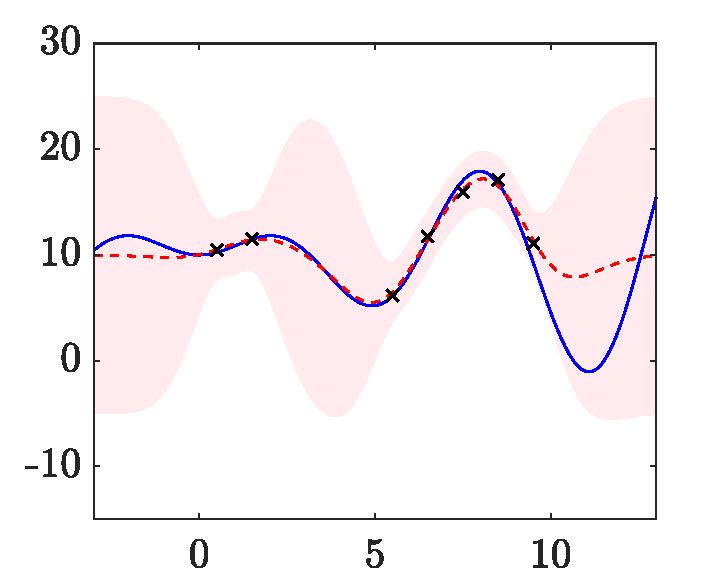
\includegraphics[width=0.49\textwidth]{../../Images/Exemple de krigeage simple 2D.pdf}
	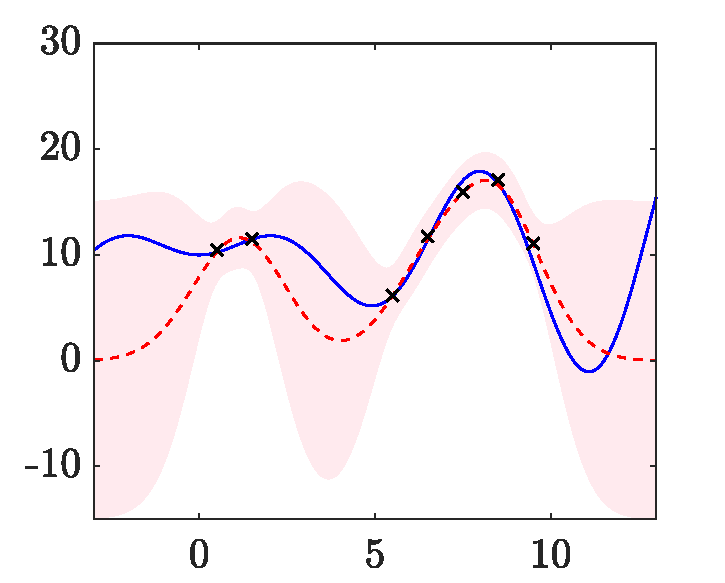
\includegraphics[width=0.49\textwidth]{../../Images/Exemple de krigeage simple à mauvaise moyenne 2D.pdf}
	\caption{Simple kriging under a correct mean function, on the left, and under a wrong one, on the right. Since $R_{\mathrm{SK}}$ does not depend on $m$ in \eqref{eq:simple_kriging_equations}, both shaded areas have the same width along the $x$-axis.}\label{fig:simple_kriging_2D}
\end{figure}

\begin{figure}[!p]
	\centering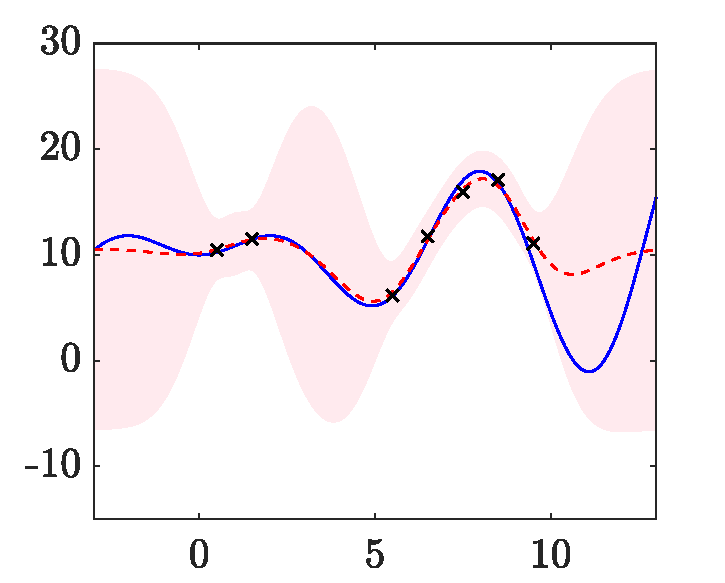
\includegraphics[width=0.49\textwidth]{../../Images/Exemple de krigeage ordinaire 2D.pdf}
	\caption{Simultaneous kriging of the training data and mean estimation by ordinary kriging. The constant mean is reconstructed here at $\hat{m}_{\mathrm{OK}}=10.56$.}\label{fig:ordinary_kriging_2D}
\end{figure}

\begin{figure}[!p]
	\centering
	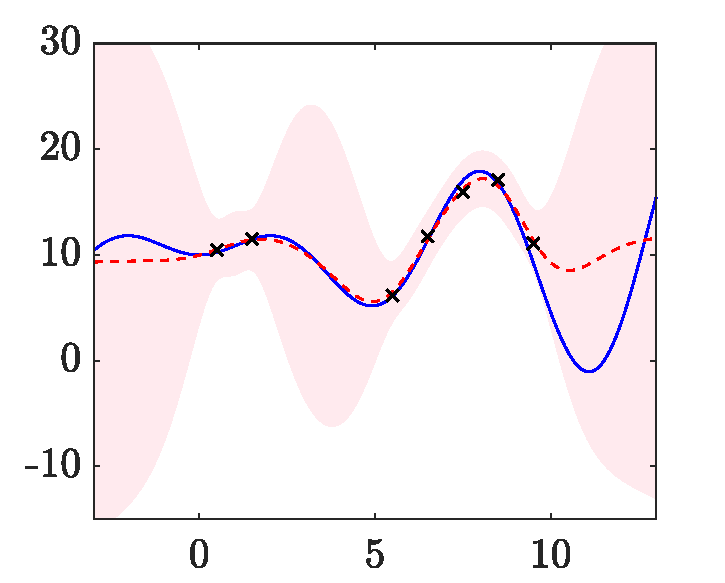
\includegraphics[width=0.49\textwidth]{../../Images/Exemple de krigeage universel 2D.pdf}
	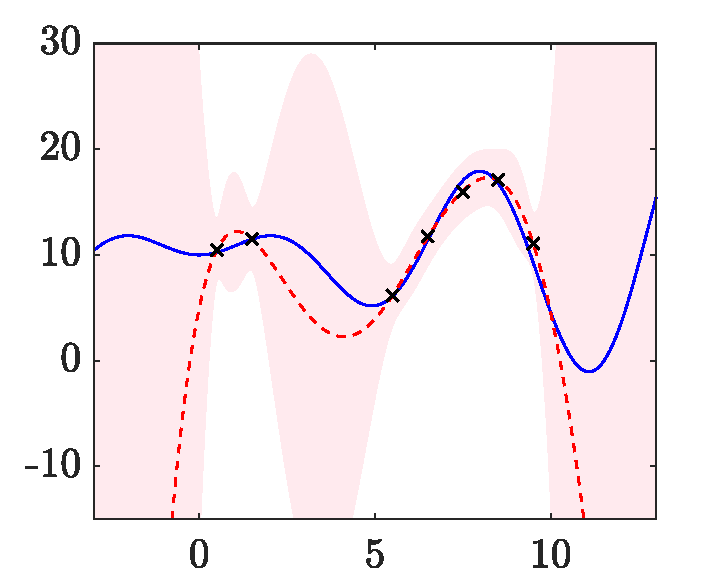
\includegraphics[width=0.49\textwidth]{../../Images/Exemple de krigeage universel à mauvaise base 2D.pdf}
	\caption{Universal kriging over an affine trend basis, on the left, and over a degree five monomial basis, on the right. The trend coefficients are estimated here at $\hat{m}_{\mathrm{UK}}=[9.78,0.15]^\top$ and $\hat{m}_{\mathrm{UK}}=[4.95,15.85,-10.82,2.40,-0.20,0.01]^\top$ respectively.}\label{fig:universal_kriging_2D}
\end{figure}

While it is the computationally simplest estimator, the SK estimator relies heavily on the prior knowledge of the mean function $m$, and poorly represents the true function in regions with a lower density of training points when that knowledge is wrong. This is particularly apparent in the gap within the training points distribution, and outside the sampled region.

As motivated by \cref{sec:kriging}, ordinary kriging tackles this issue by directly estimating a constant mean function instead of relying on a given prior. Its behaviour is similar to that of the SK estimator with the correct mean function, at the cost of a slightly increased confidence interval. This is due to the additional uncertainty associated with estimating the mean, and is quantified latter in this section.

For universal kriging, we considered polynomial means of degree $1$ and $5$. The affine basis behaves much like ordinary kriging, which it extends by a single coefficient. The affine UK envelope is barely wider than that of OK near the samples but grows faster outside the interpolation domain.

On the other hand, the degree $5$ model overfits the seven training points with six coefficients, which causes the corresponding estimator to diverge from the true function farther away from the training data. This is reflected in the UK covariance, which indicates high uncertainty in poorly sampled regions.

Since the training observations are noisy, a single draw of $\tilde{\mathbf{z}}$ cannot accurately represent the performance of the estimators above. To alleviate this issue, the training observations are redrawn over $n_\mathrm{MC}=1000$ Monte Carlo simulations, in order to compute the root mean squared error (RMSE):
\begin{equation}
	\mathrm{RMSE}_{\hat{z}_{\mathrm{K}}}:x\mapsto\sqrt{\frac{1}{n_\mathrm{MC}}\sum_{i=1}^{n_\mathrm{MC}}\|\hat{z}_{\mathrm{K}}\left(x,\tilde{\mathbf{x}},\tilde{\mathbf{z}}^{(i)};m,g\right)-h(x)\|_2^2}\label{eq:kriging_RMSE}
\end{equation}
of the estimators, where $\tilde{\mathbf{z}}^{(i)}$ denotes the $i$-th draw of the training observations.

Their average RMSE (ARMSE):
\begin{equation}
	\mathrm{ARMSE}_{\hat{z}_{\mathrm{K}}}(E)\triangleq\frac{\displaystyle\int_E{\mathrm{RMSE}_{\hat{z}_{\mathrm{K}}}(x)\:dx}}{\displaystyle\int_E{dx}}\label{eq:kriging_ARMSE}
\end{equation}
is then computed over three subsets:
\begin{equation}
	\left\{\begin{aligned}
	E_\mathrm{in}&\triangleq[0.5,1.5]\cup[5.5,9.5]\\
	E_\mathrm{gap}&\triangleq[1.5,5.5]\\
	E_\mathrm{out}&\triangleq[-3,0.5]\cup[9.5,13]
	\end{aligned}\right.
\end{equation}
of the prediction domain, as presented in \Cref{tab:kriging_rmse}.

\begin{table}[!htb]
	\centering% Generated by krigeage_2D.m, do not edit by hand.
% Each metric is averaged separately over 3 regions of the grid.
% Errors are pooled over 1000 noise realisations. The declared covariances are the same for all of them,
% since no kriging covariance involves the observations.

\begin{tabular}{|l|ccc|}\hline
Estimator & \multicolumn{3}{c|}{ARMSE}\\\hline
& in & gap & out \\\hline
Simple, correct mean & 0.85 & 1.15 & 3.23\\\hline
Simple, wrong mean & 0.87 & 3.69 & 5.88\\\hline
Ordinary & 0.85 & 1.26 & 3.25\\\hline
Universal, affine & 0.85 & 1.25 & 3.54\\\hline
Universal, degree $5$ & 0.98 & 4.02 & 70.88\\\hline
\end{tabular}

	\caption{ARMSE of the five estimators over the three subsets $E_\mathrm{in}$, $E_\mathrm{gap}$, and $E_\mathrm{out}$ of the prediction domain.}\label{tab:kriging_rmse}
\end{table}

All five estimators perform similarly in the densely sampled region, their ARMSE values ranging from $0.85$ to $0.87$, with the exception of the overfitted UK estimator. In this region, the high density of training data limits the influence of the mean on the estimation, and is thus not informative for assessing the individual impact of each estimator.

In the gap region, the choice of mean becomes more influential due to the sparsity of training points. The SK estimator with the correct mean achieves an ARMSE of $1.15$, while using an incorrect one increases the error to $3.69$. In contrast, both the OK and affine UK estimators remain close to the correctly informed SK estimator, with an increase of less than $10\%$ in ARMSE. The degree $5$ UK estimator performs worst, its ARMSE representing a $250\%$ increase over that of the correct SK estimator.

This tendency suggests that estimating the mean from the available observations generally makes the estimator more robust, provided that the mean model does not overfit the data. It is even more pronounced in the extrapolation region, where the SK estimator with an incorrect mean, and especially the high-order UK estimator, show a substantial increase in ARMSE compared with the three other estimators. However, this robustness comes at a cost, as neither the OK nor the affine UK estimator ever outperforms a correctly informed simple kriging.

Although the previous results highlight the differences in point-estimation accuracy between the five estimators, a key advantage of kriging is its ability to quantify the corresponding uncertainty. \Cref{tab:kriging_covariance} compares the confidence intervals and the contribution of the mean estimation to the overall covariance for the five estimators.

\begin{table}[!htb]
	\centering% Generated by figures_chapitre_4.m, do not edit by hand.
% Each metric is averaged separately over 3 regions of the grid.
% Errors are pooled over 1000 noise realisations. The declared covariances are the same for all of them,
% since no kriging covariance involves the observations.

\begin{tabular}{|l|ccc|ccc|}\hline
Estimator & \multicolumn{3}{c|}{Confidence half-width} & \multicolumn{3}{c|}{$R_{\hat{m}}/R_{\mathrm{K}}$}\\\hline
& in & gap & out & in & gap & out \\\hline
Simple, correct mean & 2.71 & 9.05 & 11.58 & 0.0\% & 0.0\% & 0.0\%\\\hline
Simple, wrong mean & 2.71 & 9.05 & 11.58 & 0.0\% & 0.0\% & 0.0\%\\\hline
Ordinary & 2.71 & 9.55 & 12.73 & 0.4\% & 8.9\% & 15.0\%\\\hline
Universal, affine & 2.72 & 9.74 & 16.55 & 0.8\% & 11.9\% & 43.0\%\\\hline
Universal, degree $5$ & 3.22 & 15.70 & 320.03 & 20.5\% & 59.6\% & 94.5\%\\\hline
\end{tabular}

	\caption{Average confidence interval half-width and average share of the covariance caused by the estimation of the mean for the five estimators over each region. The share is computed as the pointwise ratio of $R_{\hat{m}}$ over $R_{\mathrm{K}}=R_{\hat{m}}+R_{\mathrm{SK}}$.}\label{tab:kriging_covariance}
\end{table}

This table confirms the trend observed in the ARMSE results, as the average confidence intervals also increase with distance from the training points. As shown by the first row, the kriging covariance grows on its own, since the lack of close samples causes the estimator to rely more on its mean. In such regions, the estimated mean becomes more influential, and thus accounts for an increasing share of the total uncertainty.

Furthermore, it must be noted that both SK confidence intervals are the same, showing that simple kriging is unable to account for an incorrectly specified prior mean. Both present a half-width of $9.05$ in the gap, well inside the sampled range, although their ARMSE differ by a factor of three. This issue is particularly relevant in autonomous navigation scenarios, as a poorly informed SK estimator will be overconfident, resulting in skewed likelihood peaks. This, in turn, may lead to relevant particles being discarded while incorrect ones are retained, and so simple kriging is set aside.

Conversely, the degree $5$ UK estimator fails by trying to fit six trend coefficients to only seven training points. Outside the sampled range, the mean becomes highly uncertain, and accounts for an average of $94.5\%$ of the total covariance. Unlike simple kriging, the UK estimator propagates this uncertainty to its confidence interval, whose half-width reaches $320.03$. From a computational point of view, universal kriging requires $\tilde{n}\geq r_{\mathrm{UK}}$, and causes the matrix $g(\tilde{\mathbf{x}})^\top G(\tilde{\mathbf{x}})^{-1}g(\tilde{\mathbf{x}})$ to become ill-conditioned when the training set is too small relative to the number of trend functions.

Furthermore, every estimator requires the $\mathcal{O}(\tilde{n}^3)$ inversion of $G(\tilde{\mathbf{x}})$ once, after which, solving any related system costs $\mathcal{O}(\tilde{n}^2)$. Simple kriging thus requires an additional $\mathcal{O}(\tilde{n}^2)$ at each query point. Estimating the mean amounts to solving $r_{\mathrm{UK}}d_z$ equations, which costs $\mathcal{O}(r_{\mathrm{UK}}\:\tilde{n}^2)$ once and $\mathcal{O}(r_{\mathrm{UK}}\:\tilde{n})$ per query. The inversion of $g(\tilde{\mathbf{x}})^\top G(\tilde{\mathbf{x}})^{-1}g(\tilde{\mathbf{x}})\in\mathcal{S}_{r_{\mathrm{UK}}d_z}^{++}(\mathbb{R})$ does not depend on $\tilde{n}$, and is negligible as soon as $r_{\mathrm{UK}}d_z\ll\tilde{n}$. \Cref{tab:kriging_cost} gives the empirical cost of each estimator in floating-point operations (flop), for $\tilde{n}\in\{7,100,1600\}$.

\begin{table}[!htb]
	\centering% Generated by figures_chapitre_4.m, do not edit by hand.
% Closed-form flop counts, not timings, for 1 observed component(s)
% and training sets of 7, 100, 1600 points. Simple kriging estimates no mean, so its
% row is the reconstruction of the field that every estimator pays; the
% others are what estimating the mean adds to it.

\begin{tabular}{|l|ccc|ccc|}\hline
Estimator & \multicolumn{3}{c|}{Setup (flops)} & \multicolumn{3}{c|}{Per query (flops)}\\\hline
$\tilde{N}$ & $7$ & $100$ & $1600$ & $7$ & $100$ & $1600$ \\\hline
Simple & $114$ & $333$k & $1.37$G & $49$ & $10$k & $2.56$M\\\hline
Ordinary & $+112$ & $+20.2$k & $+5.12$M & $+14$ & $+200$ & $+3.2$k\\\hline
Universal, affine & $+255$ & $+40.8$k & $+10.3$M & $+28$ & $+400$ & $+6.4$k\\\hline
Universal, degree $5$ & $+1.16$k & $+127$k & $+30.8$M & $+84$ & $+1.2$k & $+19.2$k\\\hline
\end{tabular}

	\caption{Computational cost of the five estimators, split into the setup and the query costs. The simple kriging row is the cost of reconstructing the field, paid by every estimator, and the following ones are what estimating the mean adds to it. Since their cost is independent of the mean they were givenn the two simple estimators share the same row.}\label{tab:kriging_cost}
\end{table}

From $7$ to $1600$ training points, the setup cost of simple kriging rises from $114$ flops to $1.37$ Gflop, and its per-query cost from $49$ to $2.56$ Mflop. In our scenarios, every particle is a query point at each time step, so real-time constraints rule out a training set of that size. The other end of the table is no more comfortable: on seven points, the affine basis costs twice the reconstruction of the field, $255$ flops against $114$, and the degree $5$ basis ten times.

Ordinary kriging is thus retained for the remainder of this chapter. Estimating a constant mean from the observations is robust to misinformation, its ARMSE staying within $10\%$ of a correctly informed simple kriging everywhere, when a wrong mean triples the error in the gap. It also reports that estimation, the term $R_{\hat{m}_{\mathrm{OK}}}$ of \cref{th:ordinary_simple_kriging_link} rising from $0.4\%$ of the covariance near the samples to $8.9\%$ in the gap, so its confidence interval widens exactly where its accuracy degrades. Finally, the additional $d_z\times d_z$ inversion it requires is the smallest trend a kriging estimator can carry, and remains affordable at both ends of \cref{tab:kriging_cost}.

\subsection{Choosing the Kernel and its Hyperparameters}\label{sec:HP_estimation}

\textbf{TODO: à vérifier — sous-section renommée et préambule rédigé par Claude. Le corps
théorique qui suit est le tien, il n'a pas été touché.}

\Cref{sec:Gaussian_processes} leaves the kernel entirely to the modeller, its parameters
included, and that choice is made here. The Matérn family of \cref{th:Matérn} is retained, its
smoothness parameter $\nu$ governing the regularity of the realisations, a GP equipped with
$k_\nu$ being $p$ times mean-square differentiable if and only if $\nu>p$. Its limit
$\nu=+\infty$, the squared exponential kernel, therefore asserts a field whose realisations are
infinitely differentiable, an assumption no geophysical field supports. A finite $\nu$ is
required, and $\nu=\tfrac{3}{2}$ is retained, since it is the smallest half-integer smoothness
for which the field, and with it the kriging mean, remains differentiable. The closed form of
\cref{fig:Matérn} then applies, the kernel reducing to the product of an exponential and an
affine function of the distance.

Two parameters remain, the characteristic variance $\sigma_f^2$ and the correlation length $l$.
They are of a different nature from $\nu$, describing the particular field being surveyed rather
than the class it is assumed to belong to, and they are therefore estimated from the survey
itself rather than posited.

\textbf{TODO: à reprendre}

The kernel depends on hyperparameters $\theta$, such as the characteristic variance $\sigma_f^2$ and the correlation length $l$ of \cref{th:Matérn}, that must be inferred from the data. Given $\tilde{n}$ training inputs $\tilde{\mathbf{x}}$ and their noisy observations $\tilde{\mathbf{z}}$, degraded by a noise of covariance $\tilde{R}$, the standard approach maximises the marginal likelihood of the observations, a procedure known as evidence maximisation \cite{bib:Rasmussen-hyperparameters}. Writing $G_\theta\triangleq k_\theta(\tilde{\mathbf{x}},\tilde{\mathbf{x}})+I_{\tilde{n}}\otimes\tilde{R}$ for the noise-augmented Gram matrix and $\tilde{\mathbf{r}}\triangleq\tilde{\mathbf{z}}-m(\tilde{\mathbf{x}})$ for the residual to the GP mean, the observations are jointly Gaussian:
\begin{equation}
	p(\tilde{\mathbf{z}}|\tilde{\mathbf{x}},\theta)=\frac{1}{\sqrt{(2\pi)^{\tilde{n}d_z}\:\det(G_\theta)}}\:\exp\left(-\frac{1}{2}\tilde{\mathbf{r}}^\top G_\theta^{-1}\tilde{\mathbf{r}}\right)\label{eq:marginal_likelihood}
\end{equation}

\begin{proposition}[Maximum likelihood hyperparameters]
	A hyperparameter vector $\theta$ maximising \eqref{eq:marginal_likelihood} satisfies, for each component $\theta_i$:
	\begin{equation}
		\operatorname{tr}\left[\left((G_\theta^{-1}\tilde{\mathbf{r}})\:(G_\theta^{-1}\tilde{\mathbf{r}})^\top-G_\theta^{-1}\right)\:\frac{\partial G_\theta}{\partial\theta_i}\right]=0\label{eq:GP_MLE}
	\end{equation}
\end{proposition}

\begin{proof}
	Maximising \eqref{eq:marginal_likelihood} is equivalent to maximising its logarithm:
	\begin{equation}
		\ell(\theta)\triangleq\log p(\tilde{\mathbf{z}}|\tilde{\mathbf{x}},\theta)=-\frac{1}{2}\left(\tilde{\mathbf{r}}^\top G_\theta^{-1}\tilde{\mathbf{r}}+\log\det(G_\theta)\right)-\frac{\tilde{n}d_z}{2}\log(2\pi)
	\end{equation}
	A maximiser cancels every partial derivative. Using the differential of the matrix inverse, $\frac{\partial}{\partial\theta_i}G_\theta^{-1}=-G_\theta^{-1}\frac{\partial G_\theta}{\partial\theta_i}G_\theta^{-1}$, and Jacobi's formula, $\frac{\partial}{\partial\theta_i}\log\det(G_\theta)=\operatorname{tr}\left(G_\theta^{-1}\frac{\partial G_\theta}{\partial\theta_i}\right)$, it comes that:
	\begin{equation}
		\begin{aligned}
		\frac{\partial\ell}{\partial\theta_i}=0
		\iff&\:\tilde{\mathbf{r}}^\top G_\theta^{-1}\:\frac{\partial G_\theta}{\partial\theta_i}\:G_\theta^{-1}\tilde{\mathbf{r}}-\operatorname{tr}\left(G_\theta^{-1}\:\frac{\partial G_\theta}{\partial\theta_i}\right)=0\\
		\iff&\:\operatorname{tr}\left[\left((G_\theta^{-1}\tilde{\mathbf{r}})\:(G_\theta^{-1}\tilde{\mathbf{r}})^\top-G_\theta^{-1}\right)\:\frac{\partial G_\theta}{\partial\theta_i}\right]=0
		\end{aligned}
	\end{equation}
	using the cyclic property of the trace to rewrite the scalar quadratic form\\$\tilde{\mathbf{r}}^\top G_\theta^{-1}\frac{\partial G_\theta}{\partial\theta_i}G_\theta^{-1}\tilde{\mathbf{r}}$ as $\operatorname{tr}\left((G_\theta^{-1}\tilde{\mathbf{r}})\:(G_\theta^{-1}\tilde{\mathbf{r}})^\top\frac{\partial G_\theta}{\partial\theta_i}\right)$, since $G_\theta^{-1}$ is symmetric.
\end{proof}

\begin{remark}[Non-convexity]
	The log-marginal-likelihood is generally non-convex in $\theta$, so \eqref{eq:GP_MLE} is solved numerically by gradient-based optimisation \cite{bib:evidence}, and may admit several local maxima corresponding to different interpretations of the data, \textit{e.g.} a low-noise rapidly-varying field versus a high-noise slowly-varying one.
\end{remark}

\subsection{Simulation Scenario}\label{sec:scenario}

Every navigation result of this chapter is produced by the same scenario, as described in this section. The observation field represented by $h$ is a magnetic anomaly map of a $200\text{km}\times200\text{km}$ region above Mexico, and extracted from \cite{bib:carte-magnetique}. The map is sampled on a regular grid of $201\times201$ points with a resolution of $1\text{km}\times1\text{km}$, and is read by a bilinear interpolation between the points.

From this map are extracted $\tilde{n}$ training samples $(\tilde{\mathbf{x}},\tilde{\mathbf{z}})$, where $\tilde{\mathbf{x}}$ is sampled from a regular grid, each node being independently jittered by up to $30\%$ of the grid resolution along both axes. The grid resolution is varied from $2.5$km to $7.5$km, with increments of $1$km. This corresponds to $\tilde{n}\in\{79^2,56^2,44^2,36^2,30^2,26^2\}$. The corresponding observations $\tilde{\mathbf{z}}$ are corrupted by a Gaussian white noise of variance $\tilde{R}=10^2\text{nT}^2$. The irregular grid models navigation errors during the prior survey mission, while the white noise represents the imperfect measurements of a real sensor.

The vehicle flies over the map at a constant speed of $500$m/s along a mower pattern consisting of three parallel branches, each $80$km long, and connected by half-turns with a radius of $25.5$km. The trajectory is sampled every $\Delta_t=5$s, and lasts $n_\mathrm{steps}=150$ steps. A single time step thus covers $2.50$km.

The vehicle state consists of its horizontal position and velocity:
\begin{equation}
	x_k=\begin{bmatrix}
	p_k^{(x)}&p_k^{(y)}&v_k^{(x)}&v_k^{(y)}
	\end{bmatrix}^\top,\qquad d_x=4
\end{equation}
and its propagation is degraded with a Gaussian white noise of covariance matrix:
\begin{equation}
	Q_k=\begin{bmatrix}
	100^2&0&0&0\\
	0&100^2&0&0\\
	0&0&1^2&0\\
	0&0&0&1^2\\
	\end{bmatrix}
\end{equation}
whose position and velocity entries are respectively expressed in $\text{m}^2$ and $\text{m}^2\text{s}^{-2}$.

The observation function is the scalar ($d_z=1$) OK estimation of the magnetic anomaly field, conditioned on the $\tilde{n}$ training points, and degraded by a Gaussian white noise of covariance $R_k=5^2\text{nT}^2$. The chosen kernel is a Matérn kernel with smoothness $\nu=3/2$, which corresponds to the smallest half-integer for which the field and the kriging mean are differentiable. A bilinear observation function on the same samples is also used as comparison.

The filter is an RPF, initialised on a cloud of $N=5000$ particles, drawn around a point itself drawn from $\mathcal{N}(x_0,P_0)$, with:
\begin{equation}
	P_0=\begin{bmatrix}
	8000^2&0&0&0\\
	0&8000^2&0&0\\
	0&0&2^2&0\\
	0&0&0&2^2\\
	\end{bmatrix}
\end{equation}
in the same units, to prevent the particle cloud from being centred on the true initial state. The resampling threshold is fixed to $N_\mathrm{th}=0.5N$, and the regularisation coefficient is $\alpha_\mathrm{reg}=0.3$. This scenario is summarised by \Cref{tab:scenario}, and illustrated by \Cref{fig:magnetic_anomaly_map}.

\begin{figure}[!htb]
	\centering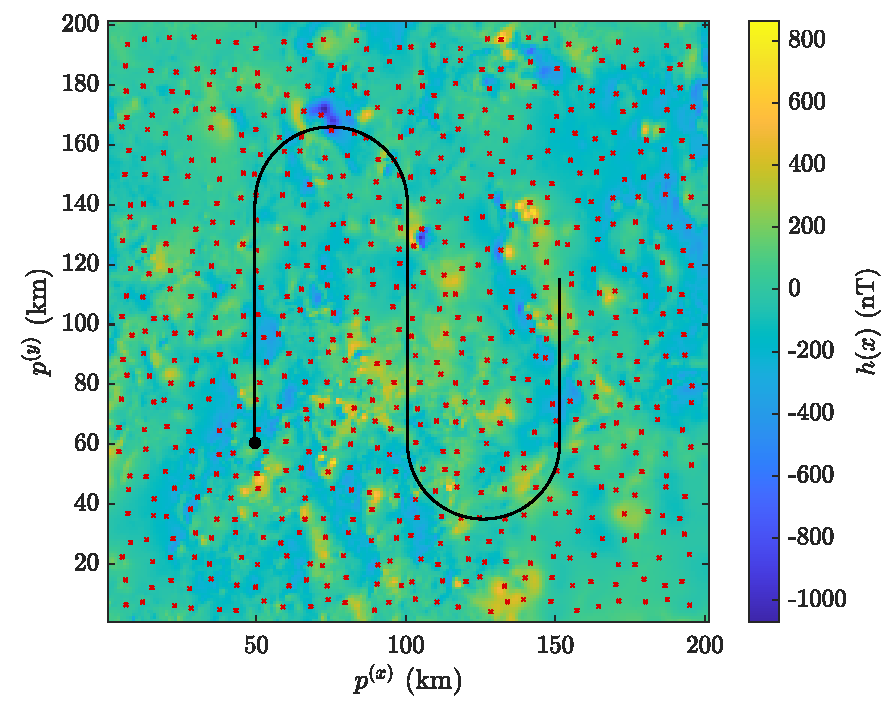
\includegraphics[width=\textwidth]{../../Images/Carte anomalie magnetique.pdf}
	\caption{The magnetic field anomaly used throughout this chapter. The black line represents the overflown trajectory, and the red crosses correspond to the training points on a $7.5$km-resolution grid.}\label{fig:magnetic_anomaly_map}
\end{figure}

\begin{table}[!htb]
	\centering
	\begin{tabular}{|l|l|l|}\hline
		\multirow{2}{*}{Map}&Surface&$200\text{km}\times200\text{km}$\\\cline{2-3}
		&Resolution&$1\text{km}\times1\text{km}$\\\hline
		\multirow{5}{*}{Kriging}&Samples&Jittered grid\\\cline{2-3}
		&Jitter&$0.3\times$Resolution\\\cline{2-3}
		&Resolution&$\in\{2.5,3.5,\dots,7.5\}$km\\\cline{2-3}
		&$\tilde{n}$&$\in\{79^2,56^2,44^2,36^2,30^2,26^2\}$\\\cline{2-3}
		&$\tilde{R}$&$10^2\text{nT}^2$\\\hline
		\multirow{6}{*}{Trajectory}&Form&$3$-branch mower\\\cline{2-3}
		&Branch length&$80$km\\\cline{2-3}
		&Turn radius&$25.5\text{km}$\\\cline{2-3}
		&Speed&$500\text{m/s}$\\\cline{2-3}
		&$\Delta_t$&$5\text{s}$\\\cline{2-3}
		&$n_\mathrm{steps}$&$150$\\\hline
		\multirow{3}{*}{State}&$d_x$&$4$\\\cline{2-3}
		&$x_k$&$\left[p_k^{(x)},p_k^{(y)},v_k^{(x)},v_k^{(y)}\right]^\top$\rule[-4mm]{0pt}{11mm}\\\cline{2-3}
		&$Q_k$&$100^2\text{m}^2$, $1^2\text{m}^2\text{s}^{-2}$\\\hline
		\multirow{4}{*}{Observation}&$d_z$&$1$\\\cline{2-3}
		&Function&OK or bilinear\\\cline{2-3}
		&Kriging kernel&Matérn, $\nu=3/2$\\\cline{2-3}
		&$R_k$&$5^2\text{nT}^2$\\\hline
		\multirow{5}{*}{Filter}&Filter&RPF\\\cline{2-3}
		&$N$&$5000$\\\cline{2-3}
		&$N_\mathrm{th}$&$0.5N$\\\cline{2-3}
		&$\alpha_\mathrm{reg}$&$0.3$\\\cline{2-3}
		&$P_0$&$8000^2\text{m}^2$, $2^2\text{m}^2\text{s}^{-2}$\\\hline
	\end{tabular}
	\caption{Simulation parameters for the navigation scenario. For improved readability, covariance matrices are represented by their diagonal coefficients only.}\label{tab:scenario}
\end{table}

Each configuration is run over $n_\mathrm{MC}=1000$ Monte Carlo realisations, redrawing the initial state and white noises. The training data are also redrawn every $10$ runs so that the metrics are averaged over the reconstruction as well as the trajectory. The performance of each one is read through two quantities:
\begin{itemize}
	\item The estimation RMSE, defined as:
	\begin{equation}
		\mathrm{RMSE}_{\hat{x}}:k\mapsto\sqrt{\frac{1}{n_\mathrm{MC}}\sum_{i=1}^{n_\mathrm{MC}}\left\|\hat{x}_k^{(i)}-x_k\right\|_2^2}
	\end{equation}
	where $\hat{x}_k^{(i)}$ is the state estimated by the $i$-th filter at time $k$, and $x_k$ is the true state at time $k$. This metric gives an absolute value for the average error made by the filter
	\item The normalised estimation error squared (NEES):
	\begin{equation}
		\mathrm{NEES}_{\hat{x}}:k\mapsto\frac{1}{n_\mathrm{MC}\:d_x}\sum_{i=1}^{n_\mathrm{MC}}\left\|\hat{x}_k^{(i)}-x_k\right\|_{\hat{P}_k^{(i)}}
	\end{equation}
	where $\|\cdot\|_{\hat{P}_k^{(i)}}$ is the Mahalanobis norm associated with the error covariance:
	\begin{equation}
		\left\|\hat{x}_k^{(i)}-x_k\right\|_{\hat{P}_k^{(i)}}\triangleq\left(\hat{x}_k^{(i)}-x_k\right)^\top\left(\hat{P}_k^{(i)}\right)^{-1}\left(\hat{x}_k^{(i)}-x_k\right)\label{eq:Mahalanobis_norm}
	\end{equation}

	This metric detects overconfident filters by using the Mahalanobis norm associated with the error covariance matrix rather than the standard Euclidean distance.
\end{itemize}

Similarly, a run is declared convergent under two different criteria, as each describes a different behaviour:
\begin{itemize}
	\item A fixed threshold of $2000$m, under which the median over the last ten steps of a filter must be. This metric is simple to read and ensures that the estimation is relatively close to the true state. However, the threshold value is arbitrary.
	\item A Mahalanobis criterion, where the median of \eqref{eq:Mahalanobis_norm} over the last ten steps must remain under the $\operatorname{erf}(3/\sqrt{2})\approx99.73\%$ quantile of a $\chi^2$ law with $d_x$ degrees of freedom. While this criterion follows the property of a Gaussian error, it primarily assesses the consistency between the estimation error and the uncertainty reported by the filter. Consequently, a filter with a large estimation error may still satisfy this criterion if it reports a sufficiently large uncertainty.
\end{itemize}

\subsection{Numerical Results}

In this section, we compare the performance of the filter using $13$ different observation functions:
\begin{itemize}
	\item The first configuration corresponds to the known map, and serves as a reference case.
	\item The six next use ordinary kriging at different grid resolutions.
	\item The final six instead use bilinear interpolation on the same grid.
\end{itemize}

Before analysing the filters themselves, it is important to assess the quality of the reconstructed maps. \Cref{fig:reconstruction_ARMSE} presents the reconstruction ARMSE along the true trajectory for ordinary kriging and bilinear interpolation across the different grid resolutions, in the sense of \eqref{eq:kriging_ARMSE}.

\begin{figure}[!htb]
	\centering
	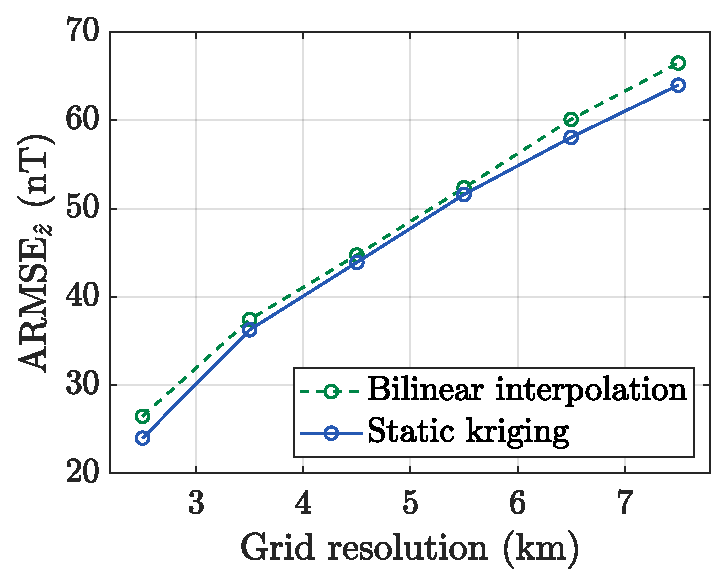
\includegraphics[width=0.6\textwidth]{../../Images/ARMSE de reconstruction.pdf}
	\caption{Reconstruction ARMSE of the field over the trajectory corridor for ordinary kriging and bilinear interpolation as a function of the training grid resolution. The domain $E$ considered is a rectangular corridor around the true trajectory, with a $28km$ margin. It covers $74\%$ of the map.}\label{fig:reconstruction_ARMSE}
\end{figure}

As one could have expected, denser grids lead to better reconstructions, the ARMSE evolving as the logarithm of the grid resolution. However, kriging and bilinear interpolation exhibit similar errors, within $1$nT of each other at every resolution but the finest. Thus, the advantage of kriging cannot be primarily attributed to the reconstruction accuracy alone.

Focusing now on the filter performance, \Cref{fig:kriging_RMSE,fig:kriging_NEES} respectively compare the RMSE and NEES of the filter using the true map, kriging and bilinear interpolation on each of the six grid resolutions. For the sake of readability, both metrics are only computed on the converged runs with respect to the threshold criterion.

\begin{figure}[!p]
	\centering
	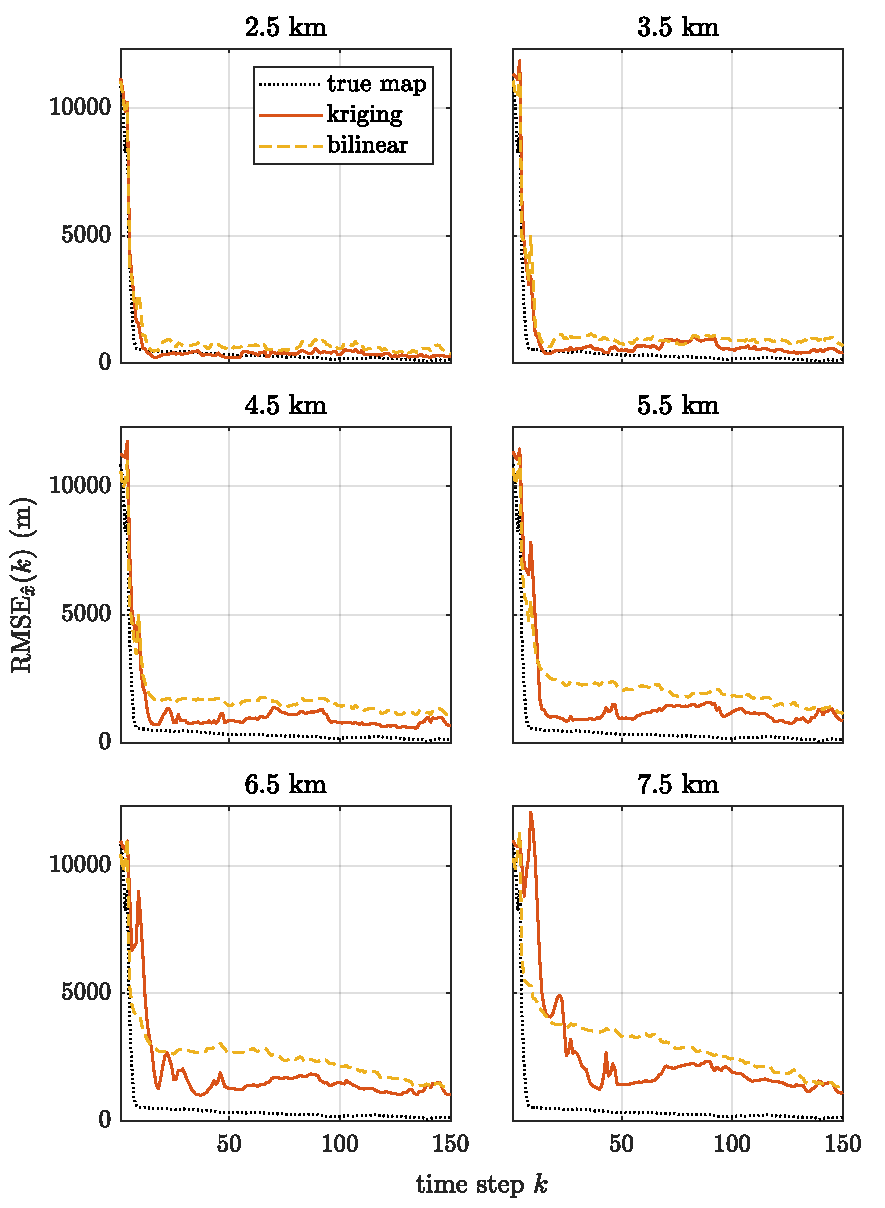
\includegraphics[width=\textwidth]{../../Images/RMSE par maille.pdf}
	\caption{Estimation RMSE for the $13$ configurations. Each panel corresponds to a different grid resolution, and the true map result is repeated for comparison.}\label{fig:kriging_RMSE}
\end{figure}

\begin{figure}[!p]
	\centering
	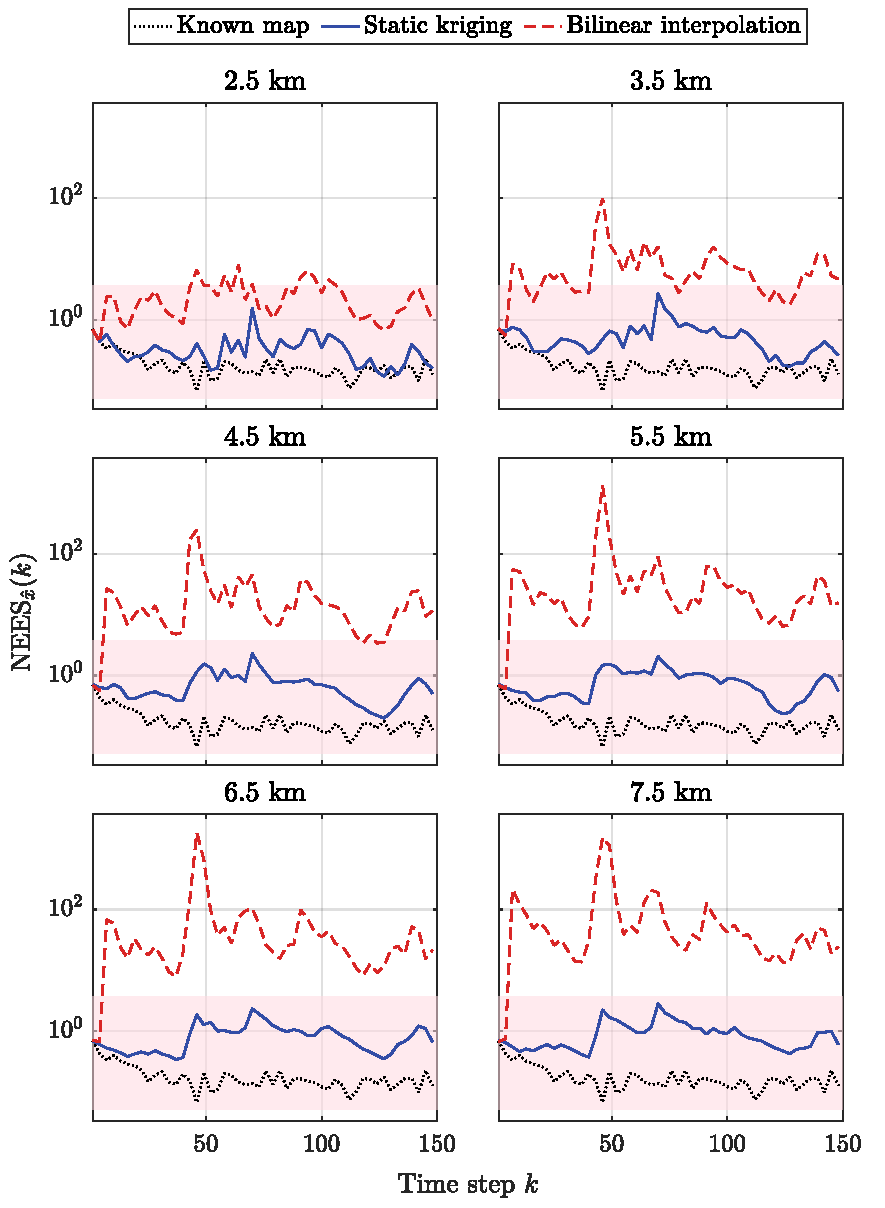
\includegraphics[width=\textwidth]{../../Images/NEES par maille.pdf}
	\caption{Estimation NEES for the $13$ configurations. The shaded area delimits the quantiles of a $\chi^2$ law with $d_x$ degrees of freedom, within which the NEES of a consistent filter falls with probability $0.99$.}\label{fig:kriging_NEES}
\end{figure}

Three main results can be drawn from the RMSE curves. First, filters with access to more training points from a denser grid achieve better performance, with the limit case of the filter using the true map outperforming every other configuration. Second, kriging-based filters consistently achieve lower RMSEs than their bilinear counterparts despite having similar map reconstruction accuracy. This result, combined with \Cref{fig:reconstruction_ARMSE}, indicates that the advantage of kriging lies in its ability to quantify reconstruction uncertainty through its covariance matrix. Finally, the time required to reach a stable estimation error increases from $13$ to $25$ steps as the grid resolution decreases from $2.5$ to $7.5$ km.

The NEES curves further highlight the superiority of kriging methods by taking the estimated error covariance matrix into account. Kriging-based filters stay within the consistency band at every resolution, whereas bilinear interpolation lies above it even on the densest map. This shows that kriging not only leads to more accurate state estimates than bilinear interpolation, but also provides a better characterisation of their associated uncertainty.

In terms of convergence rates, \Cref{fig:erreur_maille} starts by extracting the relevant the median errors from the previous curves, and \Cref{fig:convergence_maille} computes the associated convergence rates using the two metrics introduced at the beginning of this section.

\begin{figure}[!htb]
	\centering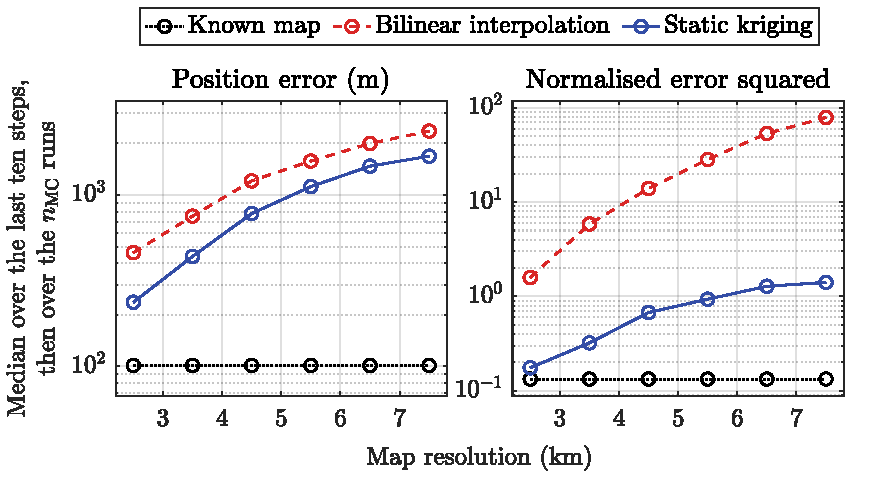
\includegraphics[width=\textwidth]{../../Images/Erreur finale par maille.pdf}
	\caption{Average median RMSE and NEES at the end of the flight for each grid resolution. These metrics are used to determine whether a run has converged.}\label{fig:erreur_maille}
\end{figure}

\begin{figure}[!htb]
	\centering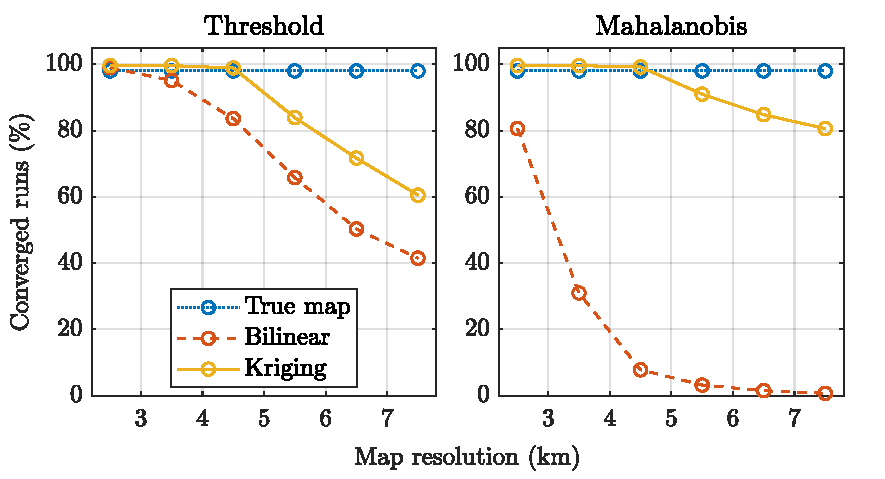
\includegraphics[width=\textwidth]{../../Images/Convergence par maille.pdf}
	\caption{Percentage of converged runs against the grid resolution for the two metrics. The true map does not depend on the resolution, and has a convergence rate of $98\%$ under both criteria.}\label{fig:convergence_maille}
\end{figure}

The first two figures show that the bilinear to kriging RMSE ratio ranges from $1.4$ to $1.9$, and increases to $9$ to $56$ for the NEES. Furthermore, while the RMSE ratio tends to decrease at lower grid resolutions, the NEES ratio follows the opposite trend. Bilinear interpolation thus completely fails to measure its accuracy at lower resolutions, while kriging degrades in step with its own accuracy.

The convergence rates follow the same pattern. Under the threshold criterion, the rate for kriging decreases from $100\%$ to $60\%$ as the grid resolution decreases, while that of bilinear interpolation decreases from $99$ to $42\%$. The two thus remain comparable. Under the Mahalanobis criterion, however, kriging only falls to $81\%$ while bilinear interpolation collapses to $1\%$, having lost every run whose reported uncertainty is consistent with its error.

However, the advantages of kriging come at an increased computational and memory costs, as described by \Cref{tab:cout_maille}.

\begin{table}[!htb]
	\centering% Generated by figures_campagnes.m, do not edit by hand.
% Analytic flop counts per run, in Gflop, not timings, for 5000 particles over
% 150 steps. Setup solves the training system once; queries cost n^2 per
% particle and per step. The true map and the bilinear model are read in eight
% flops per query and pay no setup, hence one row each: neither depends on the
% map resolution.

\begin{tabular}{|l|cc|}\hline
Observation model & Setup (flops) & Queries (flops)\\\hline
True map & -- & $6$M\\
Bilinear & -- & $6$M\\\hline
Kriging, $2.5$km & $81$G & $29.2$T\\
Kriging, $3.5$km & $10.3$G & $7.38$T\\
Kriging, $4.5$km & $2.42$G & $2.81$T\\
Kriging, $5.5$km & $726$M & $1.26$T\\
Kriging, $6.5$km & $243$M & $608$G\\
Kriging, $7.5$km & $103$M & $343$G\\
\hline
\end{tabular}

	\caption{}\label{tab:cout_maille}
\end{table}

While the setup cost can be paid before the mission, the vehicle must still be able to store between $3.67$ and $312$MB of data, and sustain an average computational rate of $0.46$ to $38.9$Gflops/s over the navigation period. These requirements remain affordable at low grid resolutions, but these configurations result in poor navigation performance, as shown above. Increasing the grid resolution improves navigation accuracy, but quickly leads to prohibitive storage and computational requirements.
